%! Author = Len Washington III
%! Date = 2/8/24

% Preamble
\documentclass[title={Chapter 6}]{fdsn201notes}

% Packages

% Document
\begin{document}

\maketitle
\setcounter{chapter}{6}

\section{What Are Proteins?}\label{sec:what-are-proteins?}
\begin{itemize}
	\item Large, complex molecules found in the cells of all living things
	\item Critical components of all the tissues of the human body
	\item Function in metabolism, immunity, fluid balance, and nutrient transport
	\item In certain circumstances, provide energy
	\item Contain a special form of nitrogen our bodies can readily use
\end{itemize}

\section{Amino Acids}\label{sec:amino-acids}
\definition{Amino acids}{the nitrogen-containing molecules that combine to form proteins}

\subsection{Essential amino acids}\label{subsec:essential-amino-acids}
\begin{itemize}
	\item Cannot be produced by our bodies
	\item Must be obtained from food
	\item Nine of 20 amino acids in our bodies are essential
\end{itemize}

\subsection{Nonessential amino acids}\label{subsec:nonessential-amino-acids}
\begin{itemize}
	\item Can be made by our bodies
\end{itemize}

\begin{figure}[H]
	\centering
	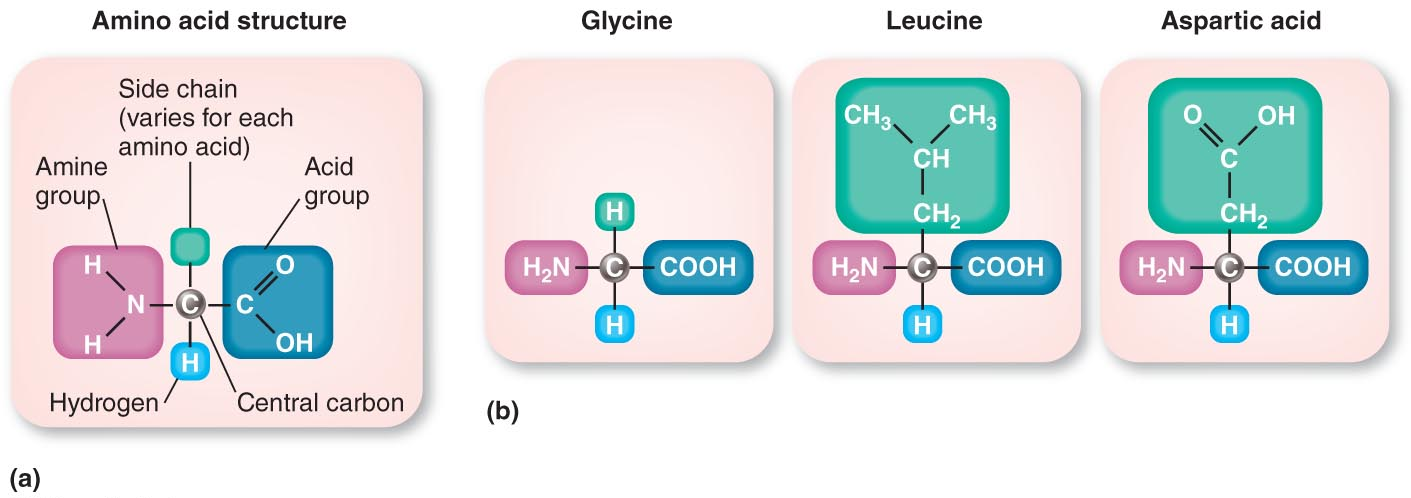
\includegraphics[width=\textwidth]{6_amino_acid}
	\caption{Structure of an Amino Acid}
	\label{fig:amino-acid-structure}
\end{figure}

\renewcommand{\arraystretch}{1.3}
\begin{table}[H]
	\centering
	\caption{Amino Acids of the Human Body}
	\label{tab:amino-acids-of-the-human-body}
	\begin{tabular}{>{\columncolor{rowlightgreen}}p{0.5\textwidth} >{\columncolor{rowmedgreen}}p{0.5\textwidth}}
		\rowcolor{rowdarkgreen}\textbf{Essential Amino Acids} & \textbf{Nonessential Amino Acids}\\
		These amino acids must be consumed in the diet. & These amino acids can be manufactured by the body.\\
		Histidine & Alanine\\
		Isoleucine & Arginine\\
		Leucine & Asparagine\\
		Lysine & Aspartic acid\\
		Methionine & Cysteine\\
		Phenylalanine & Glutamic acid\\
		Threonine & Glutamine\\
		Tryptophan & Glycine\\
		Valine & Proline\\
		& Serine\\
		& Tryosine\\
		\rowcolor{rowdarkgreen} & \\
	\end{tabular}
\end{table}

\begin{figure}[H]
	\centering
	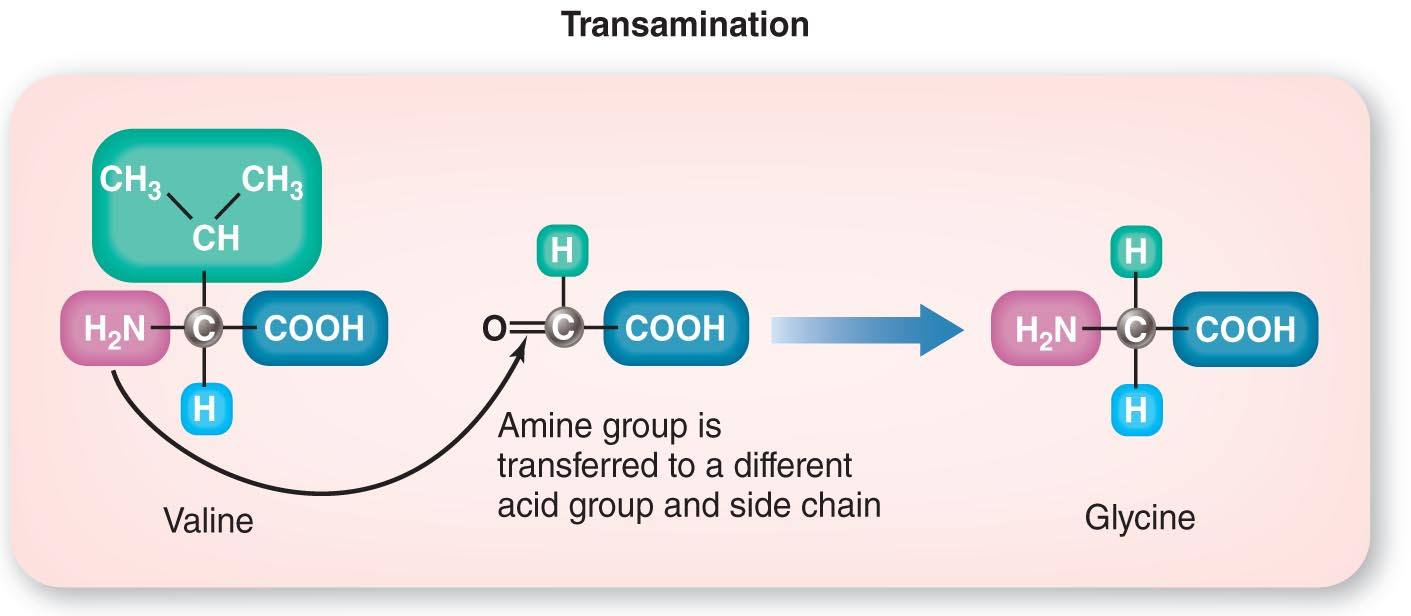
\includegraphics[width=\textwidth]{6_transamination}
	\caption{Transamination}
	\label{fig:transamination}
\end{figure}

\section{How Are Proteins Made?}\label{sec:how-are-proteins-made?}
\begin{itemize}
	\item When two amino acids join together in a peptide bond, they form a dipeptide
	\item Two or more amino acids bonded together form a polypeptide
	\item Proteins are made by combining multiple amino acids
\end{itemize}

\begin{figure}[H]
	\centering
	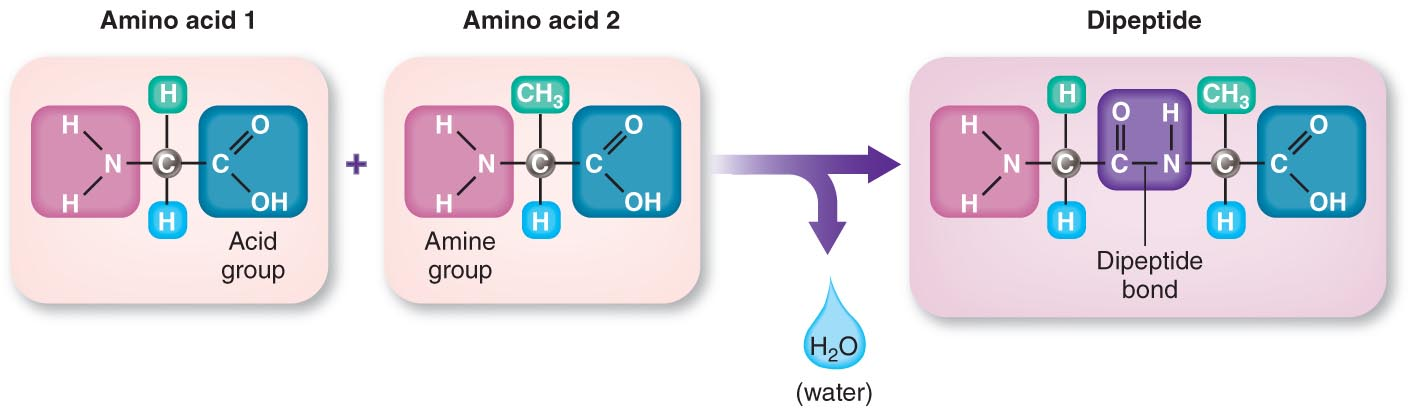
\includegraphics[width=\textwidth]{6_amino_acid_bonding}
	\caption{Amino Acid Bonding}
	\label{fig:amino-acid-bonding}
\end{figure}

\definition{Transcription}{use of the genetic information in DNA to make RNA}
\begin{itemize}
	\item mRNA copies the genetic information and carries it to the ribosome
\end{itemize}
\definition{Translation}{conversion of genetic information in RNA to assemble amino acids in the proper sequence to synthesize a protein on the ribosome}

\section{Protein Organization Determines Function}\label{sec:protein-organization-determines-function}
\begin{itemize}
	\item Protein structure has four levels
	\begin{itemize}
		\item Primary structure
		\begin{itemize}
			\item Sequential order of amino acids
		\end{itemize}
		\item Secondary structure
		\begin{itemize}
			\item Spiral shape due to the chemical bonding between the amino acids
		\end{itemize}
		\item Tertiary and quaternary structure
		\begin{itemize}
			\item Further folding into a unique three-dimensional shape that may be globular or fibrous
		\end{itemize}
	\end{itemize}
\end{itemize}

\begin{figure}[H]
	\centering
	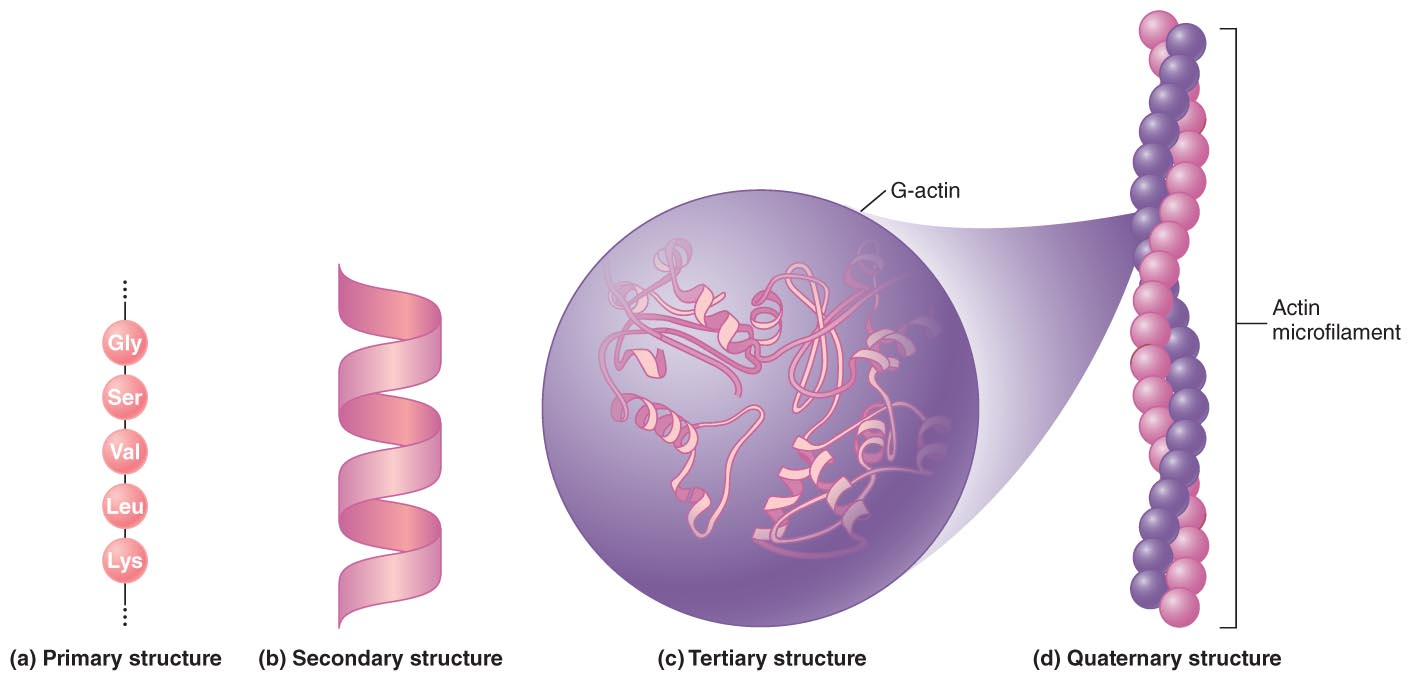
\includegraphics[width=\textwidth]{6_protein_structure}
	\caption{Levels of Protein Structure}
	\label{fig:protein-structure-leves}
\end{figure}

\section{Protein Function}\label{sec:protein-function}
\begin{itemize}
	\item Proteins lose shape (denaturation) when subject to
	\begin{itemize}
		\item Heat
		\item Acids and bases
		\item Heavy metals
		\item Alcohol
	\end{itemize}
	\item Denaturation results in an irreversible loss in protein function
\end{itemize}

\begin{figure}[H]
	\centering
	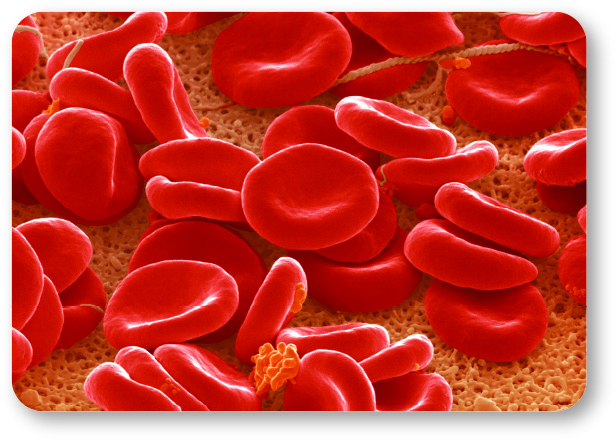
\includegraphics[width=\textwidth]{6_protein_shape_function}
	\caption{Protein Shape Determines Function}
	\label{fig:protein-shape-determines-function}
\end{figure}

\section{Protein Synthesis Can Be Limited}\label{sec:protein-synthesis-can-be-limited}
\definition{Incomplete protein}{does not contain all essential amino acids in sufficient quantites}
\begin{itemize}
	\item Growth and health are compromised
	\item Considered a ``low-quality'' protein
\end{itemize}
\definition{Complete protein}{Contains sufficient amounts of all nine essential amino acids}
\begin{itemize}
	\item Considered a ``high-quality'' protein
\end{itemize}

\section{Protein Synthesis Can Be Enhanced}\label{sec:protein-synthesis-can-be-enhanced}
\definition{Mutual supplementation}{combining two incomplete proteins to make a complete protein}\\

\definition{Complementary proteins}{two protein sources that together supply all nine essential amino acids}
\begin{itemize}
	\item Example: beans and rice
\end{itemize}

\begin{figure}[H]
	\centering
	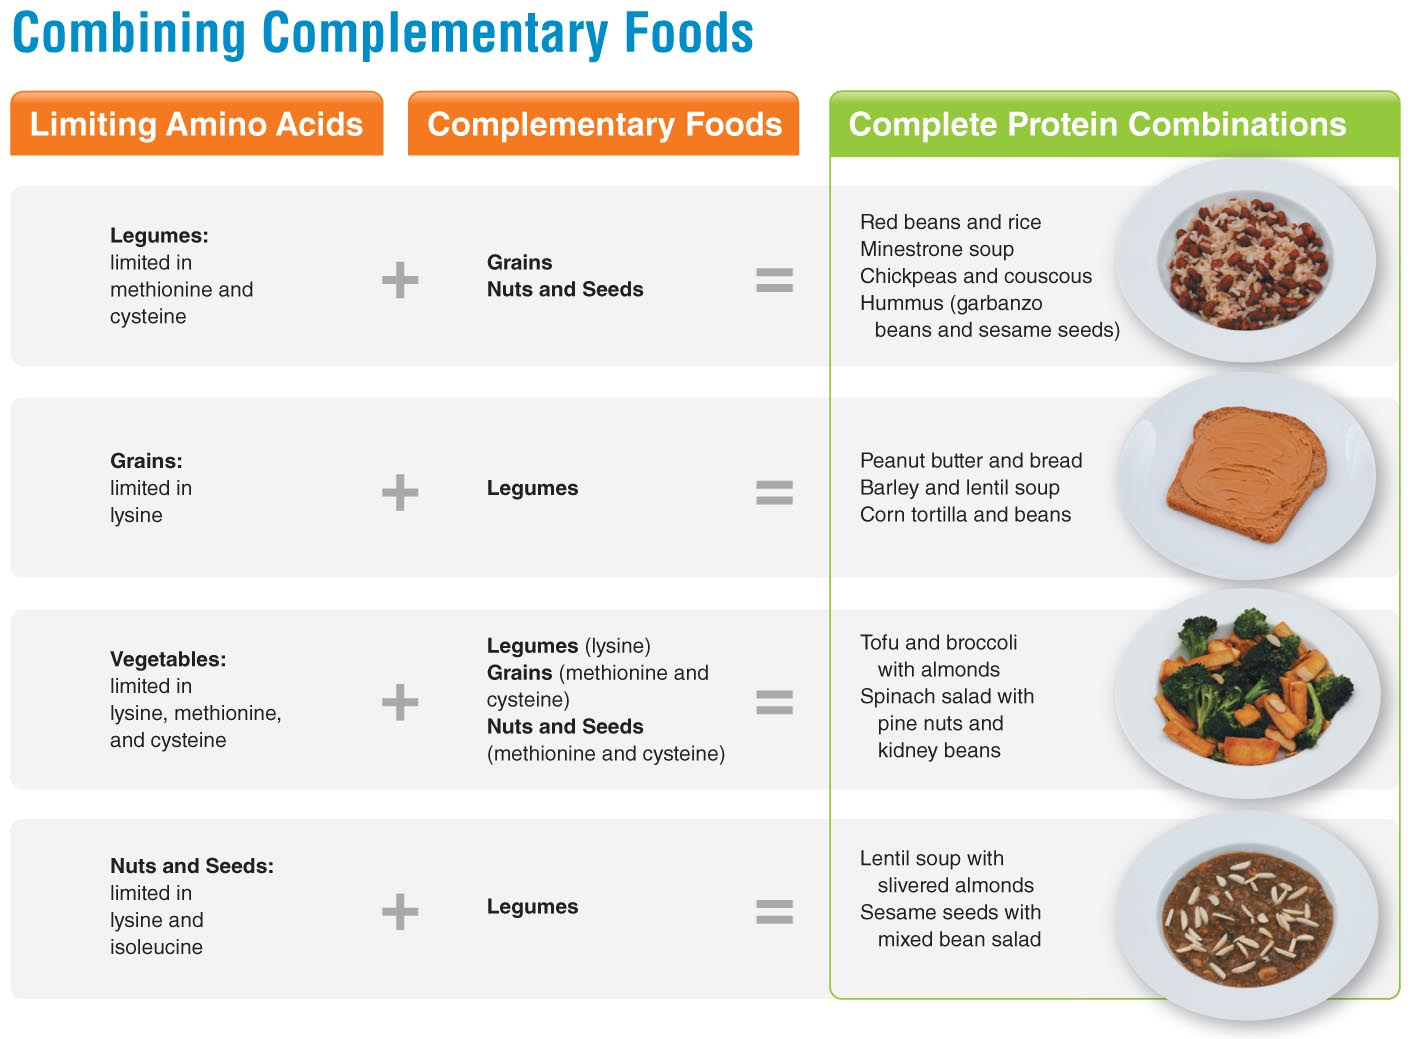
\includegraphics[width=\textwidth]{6_complementary_foods}
	\caption{Combining Complementary Foods}
	\label{fig:combining-complementary-foods}
\end{figure}

\section{Why Do We Need Proteins?}\label{sec:why-do-we-need-proteins?}
\begin{itemize}
	\item Cell growth, repair, and maintenance
	\item Enzymes
	\item Hormones
	\item Fluid and electrolyte balance
	\item pH balance
	\item Antibodies to protect against disease
	\item Energy source
	\item Transport and storage of nutrients
	\item Compounds such as neurotransmitters, fibrin, and collagen
\end{itemize}

\begin{figure}[H]
	\centering
	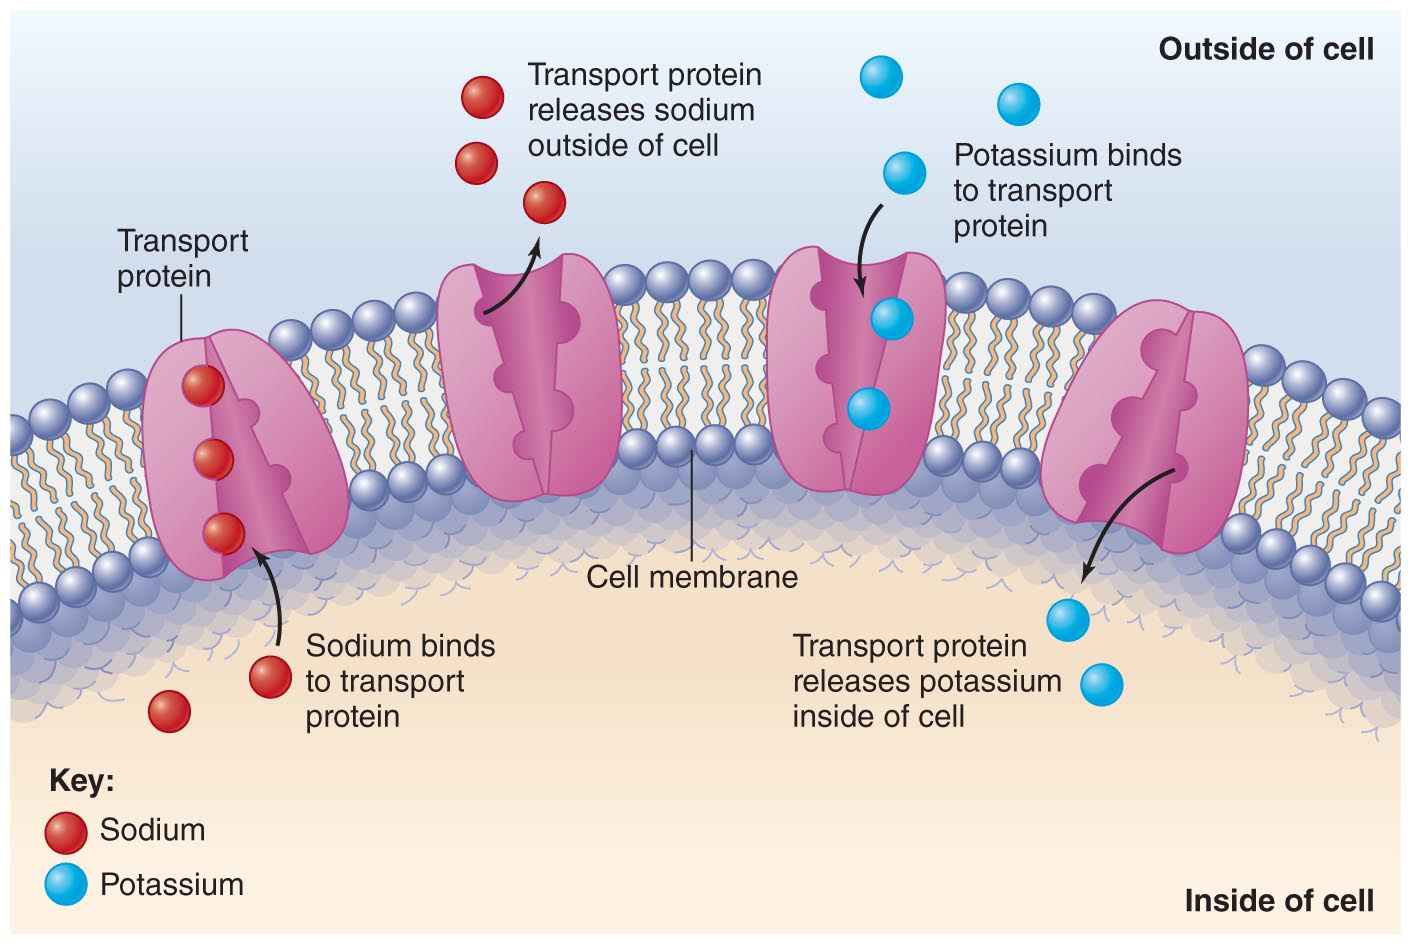
\includegraphics[width=\textwidth]{6_electrolyte_balance_proteins}
	\caption{Role of Proteins in Electrolyte Balance}
	\label{fig:role-of-proteins-in-electrolyte-balance}
\end{figure}

\section{How Do We Break Down Proteins?}\label{sec:how-do-we-break-down-proteins?}
\begin{itemize}
	\item Stomach acids and enzymes break proteins into short polypeptides
	\item Digestion of proteins continues in the small intestine, where the polypeptides are further broken down
	\begin{itemize}
		\item Pancreatic enzymes called proteases complete the digestion of proteins into single amino acids
	\end{itemize}
\end{itemize}

\begin{itemize}
	\item Protein digestibility affects protein quality
	\item Animal protein sources (meat, dairy), soy products, and legumes are highly digestible
	\item Grains and vegetable proteins are less digestible
\end{itemize}

\section{How Much Protein Should We Eat?}\label{sec:how-much-protein-should-we-eat?}
\begin{itemize}
	\item People who require more protein include
	\begin{itemize}
		\item Children
		\item Adolescents
		\item Pregnant or lactating women
		\item Athletes
		\item Vegetarians
	\end{itemize}
	\item Nitrogen balance describes the relationship between how much nitrogen (or protein) we consume and excrete each day
\end{itemize}

\begin{figure}[H]
	\centering
	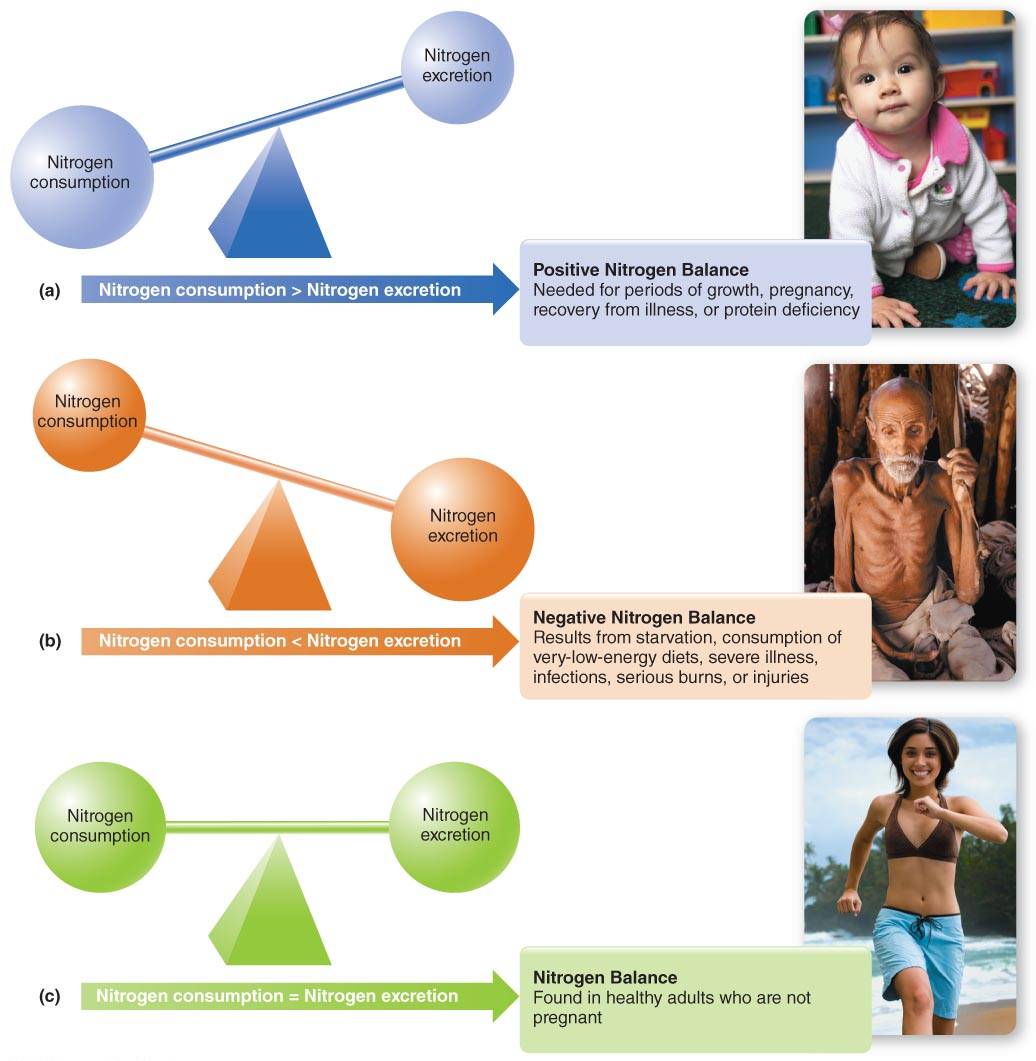
\includegraphics[width=\textwidth]{6_nitrogen_balance}
	\caption{Nitrogen Balance}
	\label{fig:nitrogen-balance}
\end{figure}

\begin{itemize}
	\item Recommended Dietary Allowance (RDA)
	\begin{itemize}
		\item 0.8 grams of protein per kilogram of body weight per day
		\item 10--35\% of total intake should be from protein
	\end{itemize}
	\item Most Americans meet or exceed the RDA for dietary protein
	\item This is true for many athletes as well
	\item Certain groups of athletes, such as distance runners, figure skaters, female gymnasts, and wrestlers who are dieting, are at risk for low protein intake
\end{itemize}

\section{Protein Sources}\label{sec:protein-sources}
\begin{itemize}
	\item Protein sources include much more than just mean
	\begin{itemize}
		\item Legumes
		\item Nuts
		\item ``New'' foods
		\begin{itemize}
			\item quorn
			\item quinoa
			\item amaranth
			\item teff
			\item millet
			\item sorghum
		\end{itemize}
	\end{itemize}
\end{itemize}

\section{Too Much Dietary Protein Can Be Harmful}\label{sec:too-much-dietary-protein-can-be-harmful}
\begin{itemize}
	\item The risks of too much dietary protein include
	\begin{itemize}
		\item High cholesterol and heart disease
		\begin{itemize}
			\item Diets high in protein from animal sources are associated with high blood cholesterol
		\end{itemize}
		\item Kidney disease
		\begin{itemize}
			\item High-protein diets are associated with an increased risk of kidney disease in people who are susceptible
		\end{itemize}
	\end{itemize}
	\item There is no evidence that high-protein diets lead to bone loss, except in people consuming inadequate calcium
\end{itemize}

\begin{figure}[H]
	\centering
	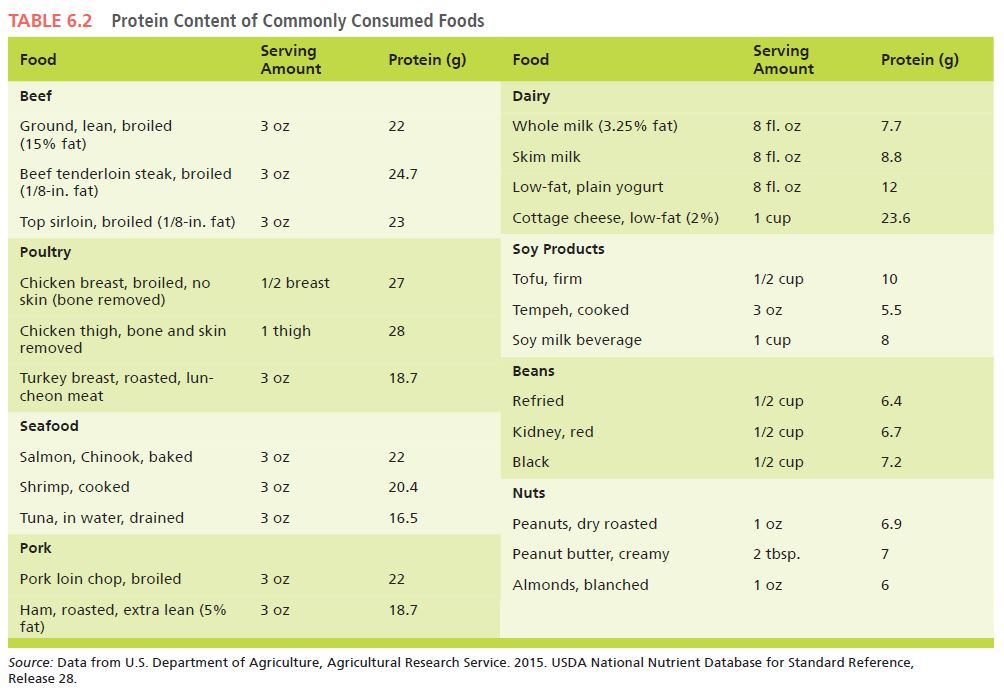
\includegraphics[width=\textwidth]{6_common_foods_protein}
	\caption{Protein Content of Common Foods}
	\label{fig:protein-content-of-common-foods}
\end{figure}

\section{Disorders Related to Protein Intake}\label{sec:disorders-related-to-protein-intake}
\definition{Protein-energy malnutrition}{a disorder caused by inadequare intake of protein and energy}
\begin{itemize}
	\item There are two common, serious forms
	\begin{itemize}
		\item Marasmus
		\item Kwashiorkor
	\end{itemize}
\end{itemize}

\subsection{Marasmus}\label{subsec:marasmus}
Disease resulting from severely inadequate intakes of protein, energy, and other nutrients
\begin{itemize}
	\item It is characterized by extreme tissue wasting and stunted growth and development
\end{itemize}

\subsection{Kwashiorkor}\label{subsec:kwashiorkor}
Disease resulting from extremely low protein intake

\begin{itemize}
	\item Kwashiorkor symptoms include
	\begin{itemize}
		\item Some weight loss and muscle wasting
		\item Edema resulting in distention of the belly
		\item Retarded growth and development
	\end{itemize}
	\item Kwashiorkor is often seen in children in developing countries
\end{itemize}

\section{Can Vegetarian Diets Provide Protein?}\label{sec:can-vegetarian-diets-provide-protein?}
\definition{Vegetarianism}{restricting the diet to foods of plant origin}
\begin{itemize}
	\item There are many versions of vegetarianism
	\item There are many reasons to adopt a vegetarian diet
\end{itemize}

\begin{table}[H]
	\centering
	\caption{Types of Vegetarian Diets}
	\label{tab:types-of-vegetarian-diets}
	\rowcolors{2}{rowmedgreen}{rowlightgreen}
	\begin{tabular}{p{0.3\textwidth} p{0.35\textwidth} p{0.35\textwidth}}
		\rowcolor{rowdarkgreen}%
		\textbf{Type of Diet} & \textbf{Foods Consumed} & \textbf{Comments}\\
		Semivegetarian (also called flexitarian or plant-based diet) & Vegetables, grains, nuts, fruits, legumes; sometimes meat, seafood, poultry, eggs and dairy products & Typically excluded or limit red meat; may also avoid other meats\\
		Pescovegetarian \\
		Lacto-ovovegetarian \\
		Lacto-vegetarian \\
		Ovovegetarian & Vegetables, grains, nuts, fruits, legumes and eggs & Excludes dairy, flesh, and seafood products\\
		\rowcolor{rowdarkgreen} & & \\
	\end{tabular}
\end{table}

\section{Why Vegetarianism?}\label{sec:why-vegetarianism?}
\begin{itemize}
	\item People chose vegetarianism because of
	\begin{itemize}
		\item Health benefits
		\item Ecological reasons
		\item Religious reasons
		\item Ethical reasons
		\item Concerns over food safety
	\end{itemize}
\end{itemize}

\section{Health Benefits of Vegetarianism}\label{sec:health-benefits-of-vegetarianism}
\begin{itemize}
	\item Lower intake of fat and total energy
	\item Lower blood pressure
	\item Reduced risk of heart disease
	\item Reduced risk of some types of cancer
	\item Fewer digestive problems
	\item Reduced risk of kidney disease, kidney stones, and gallstones
\end{itemize}

\section{Challenges of Vegetarianism}\label{sec:challenges-of-vegetarianism}
\begin{itemize}
	\item Vegetarian diets can be low in some vitamins and minerals (iron, calcium, zinc, vitamins D and $\mbox{B}_{12}$)
	\item Vegetarians must plan a balanced and adequate diet
	\item Soy products are an excellent protein source
	\item Vegetarians should include complementary proteins
	\item Vegetarians can find health eating tips for vegetarians at MyPlate online
\end{itemize}

\section{In Depth: Vitamins and Minerals}\label{sec:in-depth:-vitamins-and-minerals}
\subsection{Macronutrients}\label{subsec:macronutrients}
\begin{itemize}
	\item Carbohydrates
	\item Fats
	\item Protein
	\item Provide energy
	\item Required in relatively large amounts
\end{itemize}

\subsection{Micronutrients}\label{subsec:micronutrients}
\begin{itemize}
	\item Vitamins
	\item Minerals
	\item Do not supply energy
	\item Required in relatively small amounts
	\item Assist body functions (e.g., energy metabolism, maintenance of healthy cells and tissues)
	\item Absorption may be very low (3--10\%) when compared to macronutrients (85--99\%)
	\item Many micronutrients need to be chemically altered before they are active in the body
\end{itemize}

\subsection{Vitamins}\label{subsec:vitamins}
\begin{itemize}
	\item Organic compounds
	\item Thirteen are essential
	\item Nine are soluble in water
	\item Four are soluble in fat
\end{itemize}

\subsection{Characteristics of Fat-Soluble Vitamins}\label{subsec:characteristics-of-fat-soluble-vitamins}
\begin{itemize}
	\item Large storage capability
	\item Toxicity is possible
	\item Deficiency symptoms may take many months to develop
	\item May occur in numerous chemical forms
\end{itemize}

\subsection{Characteristics of Water-Soluble Vitamins}\label{subsec:characteristics-of-water-soluble-vitamins}
\begin{itemize}
	\item Minimal storage capacity
	\item Toxicity is rare
	\item Deficiency symptoms occur quickly
	\item Excreted in urine when tissues are saturated
\end{itemize}

\subsection{General Properties of Minerals}\label{subsec:general-properties-of-minerals}
\begin{itemize}
	\item Inorganic
	\item Cannot be synthesized by plants or animals
	\item Not digested or broken down prior to absorption
	\item Two classifications based on need
\end{itemize}

\subsection{Characteristics of Major Minerals}\label{subsec:characteristics-of-major-minerals}
\begin{itemize}
	\item Required in amounts of at least 100 mg/day
	\item Body contains 5 g or higher
	\item Seven major minerals
\end{itemize}

\subsection{Characteristics of Trace Minerals}\label{subsec:characteristics-of-trace-minerals}
\begin{itemize}
	\item Required in amounts of less than 100 mg/day
	\item Body contains less than 5 g
	\item Eight trace minerals are essential for human health
\end{itemize}

\begin{itemize}
	\item Absorption of micronutrients depends on numerous factors
	\begin{itemize}
		\item Chemical form (e.g., absorption of heme iron from meats, fish, poultry is $\sim25\%$, whereas non-heme iron from plant products is $\sim3--5\%$)
		\item Numerous factors in foods bind micronutrients and prevent absorption
		\item Other nutrients within a meal alter absorption
	\end{itemize}
	\item Supplementation of micronutrients is controversial
	\begin{itemize}
		\item Easier to develop toxicity with supplements
		\item Some may be harmful to certain subgroups of consumers
		\item Most minerals are better absorbed from animal food sources
		\item Eating a variety of foods provides many other nutrients (e.g., phytochemicals)
		\item Supplements may alter the balance between nutrients
	\end{itemize}
	\item Adequate intake of these minerals has been as been associated with lowered disease risk
	\begin{itemize}
		\item Vitamin D and colon cancer
		\item Vitamin E and complications of diabetes
		\item Vitamin K and osteoporosis
		\item Calcium and hypertension
		\item Chromium and type 2 diabetes in older adults
		\item Magnesium and muscle wasting in older adults
		\item Selenium and certain types of cancer
	\end{itemize}
	\item Do more essential micronutrients exist?
	\item Nutrition researchers continue to explore the possibility of other substances being essential
	\item Vitamin-like factors (e.g., carnitine) and numerous minerals (e.g., boron, nickel, silicon) may prove to be essential in our diet
\end{itemize}

\end{document}
